\documentclass{beamer}
\usepackage{xeCJK}
\usetheme{Copenhagen}
\usecolortheme{beaver}
\usepackage{float}
\usepackage{graphicx}
\usepackage[boxed]{algorithm2e}
\title{Skip List}
\author{Kvrmnks}
\date{\today}
\begin{document}
	\begin{frame}
		\titlepage
	\end{frame}
	\section{简介}
	\subsection{Skip List是什么}

	\begin{frame}
		\frametitle{Skip List是什么}
		\begin{figure}[H]
			\centering
			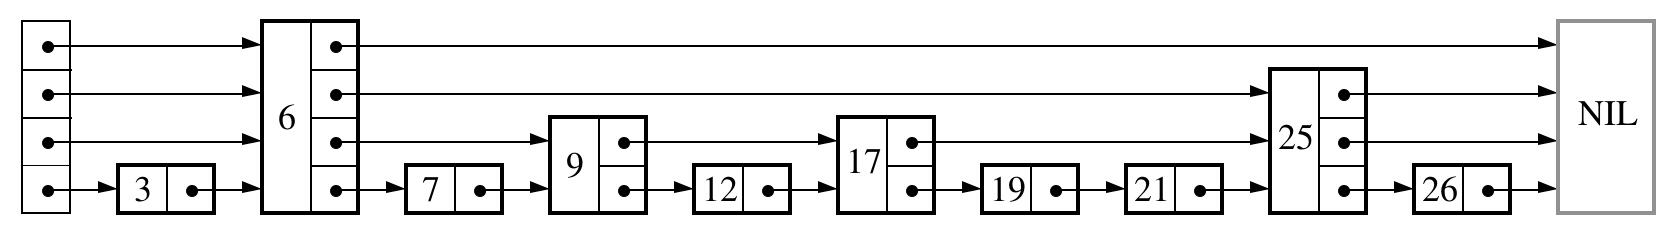
\includegraphics[scale=0.25]{./img/what_skip_list_is.jpg}
			
		\end{figure}
		\pause
		是链表,高度不一样,指针多了不少,是有序的,指针有的是跳着指的。
	\end{frame}

	\begin{frame}
		\frametitle{Skip List的功能}
		\begin{enumerate}
			\item 查找 \quad 期望$O(\log n)$,最坏$O(n)$
			\item 插入 \quad 期望$O(\log n)$,最坏$O(n)$
			\item 删除 \quad 期望$O(\log n)$,最坏$O(n)$
			\item 前驱 \quad 期望$O(\log n)$,最坏$O(n)$
			\item 后继 \quad 期望$O(\log n)$,最坏$O(n)$
			\item 第$k$大 \quad 期望$O(\log n)$,最坏$O(n)$
			\item $rank$ \quad 期望$O(\log n)$,最坏$O(n)$
			\item 空间复杂度 \quad 期望$O(n)$, 最坏$O(n\log n)$
		\end{enumerate}
	\end{frame}
	\begin{frame}
		\frametitle{先不管Skip List...}
		\begin{enumerate}
			\item 什么是期望复杂度
			\item 什么是最好复杂度
			\item 什么是最坏复杂度
			\item 什么是均摊复杂度
		\end{enumerate}
	\end{frame}

	\begin{frame}
		\frametitle{先不管Skip List...}
		\begin{enumerate}
			\item 什么是最好复杂度
			\item 什么是最坏复杂度
		\end{enumerate}
		冒泡排序
	\end{frame}

	\begin{frame}
		\frametitle{先不管Skip List...}
		\begin{enumerate}
			\item 什么是期望复杂度
			\item 什么是均摊复杂度
		\end{enumerate}
	\end{frame}

	\begin{frame}
		\frametitle{先不管Skip List...}
		为什么要关心最坏复杂度和最好复杂度?

		参数化算法 \quad 缝合怪
	\end{frame}

	\subsection{Skip List有哪些优势}
	\begin{frame}
		\frametitle{Skip List有哪些优势}
		\begin{enumerate}
			\item 实现简单
			\item 期望下有和一般的平衡树一样的复杂度
			\item 更好地支持并行
			\item finger search
		\end{enumerate}
	\end{frame}

	\section{分块}
	\subsection{怎样让链表快一点}
	\begin{frame}
		\frametitle{怎样让链表快一点}
		\begin{figure}[H]
			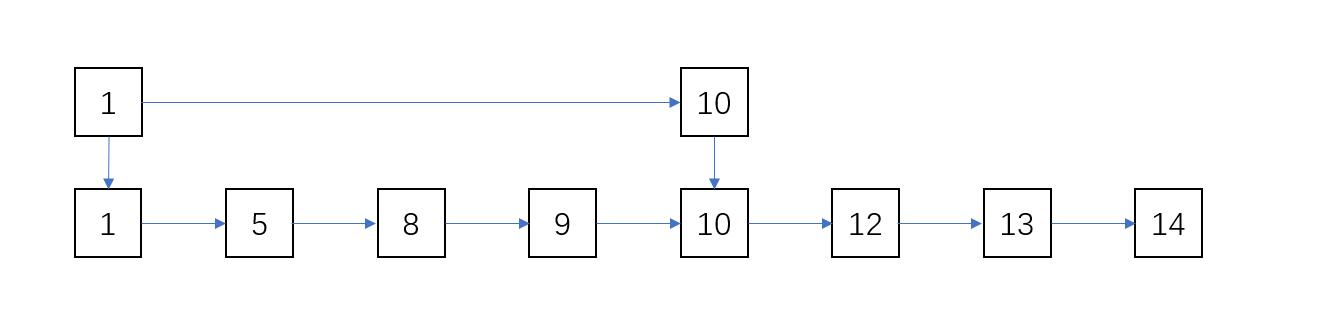
\includegraphics[scale=0.25]{./img/faster.jpg}
		\end{figure}
		\pause
		分块! \\
		\pause
		\begin{enumerate}
			\item<3-> 怎么分最好?\uncover<5->{$\sqrt{n}$分块}
			\item<4-> 支持删除插入吗?\uncover<6->{同样是$O(\sqrt{n})$的复杂度}
	\end{enumerate}
	\end{frame}
	\begin{frame}
		\frametitle{块状链表}
		假设一共有$n$个数,假设将链表分成$\frac{n}{a}$块,块的大小是$a$

		于是每次查找的复杂度是$O(\frac{n}{a}+a)$,由均值不等式$a = \sqrt{n}$时,复杂度达到最小,这时复杂度是$O(\sqrt{n})$
	\end{frame}

	\begin{frame}
		\frametitle{块状链表}
		考虑怎样维护插入和删除。\\
		\begin{figure}[H]
			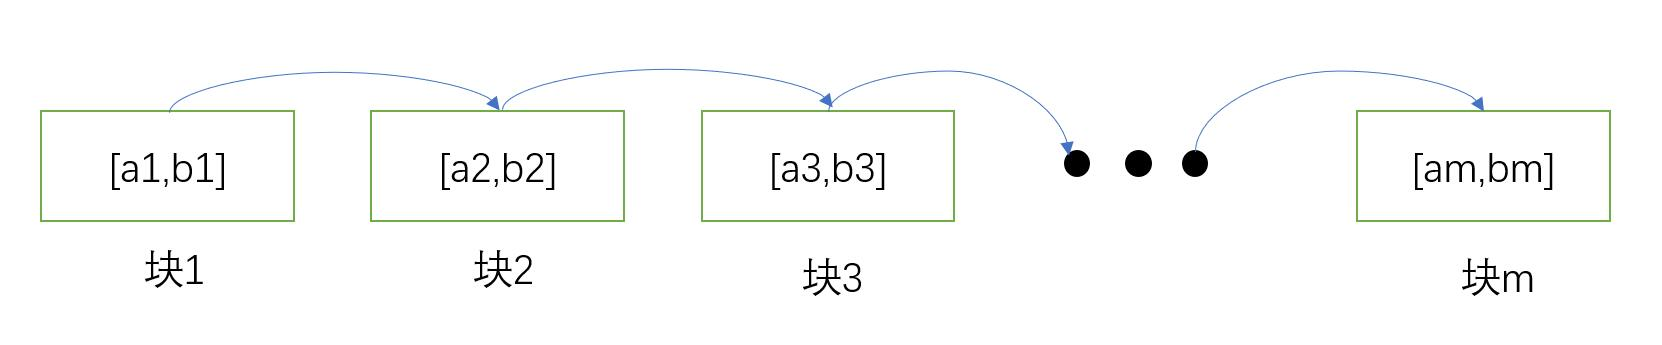
\includegraphics[scale=0.2]{./img/block.jpg}
		\end{figure}
		如果插入的块比$\sqrt{n}$,把块分裂成两个。\\
		删除直接在所在块中删除 \\
		将新相接的块尝试合并 \\
	\end{frame}

	\begin{frame}
		\frametitle{块状链表}
		假设第$i$块的大小为$s_{i}$,
		根据上面的规则有$$s_{i}+s_{i-1}\geq \sqrt{n}$$
		累加这个不等式,可以得到$$s_{1}+2*\sum_{i=2}^{m-1}s_{i}+s_{m} \geq m\sqrt{n}$$
		放缩一下得到
		$$2n\geq m\sqrt{n}$$$$m\leq 2\sqrt{n}$$
		于是总复杂度为$$O(\sqrt{n})$$
	\end{frame}
	\begin{frame}
		\frametitle{再快一点?}
		\begin{figure}[H]
			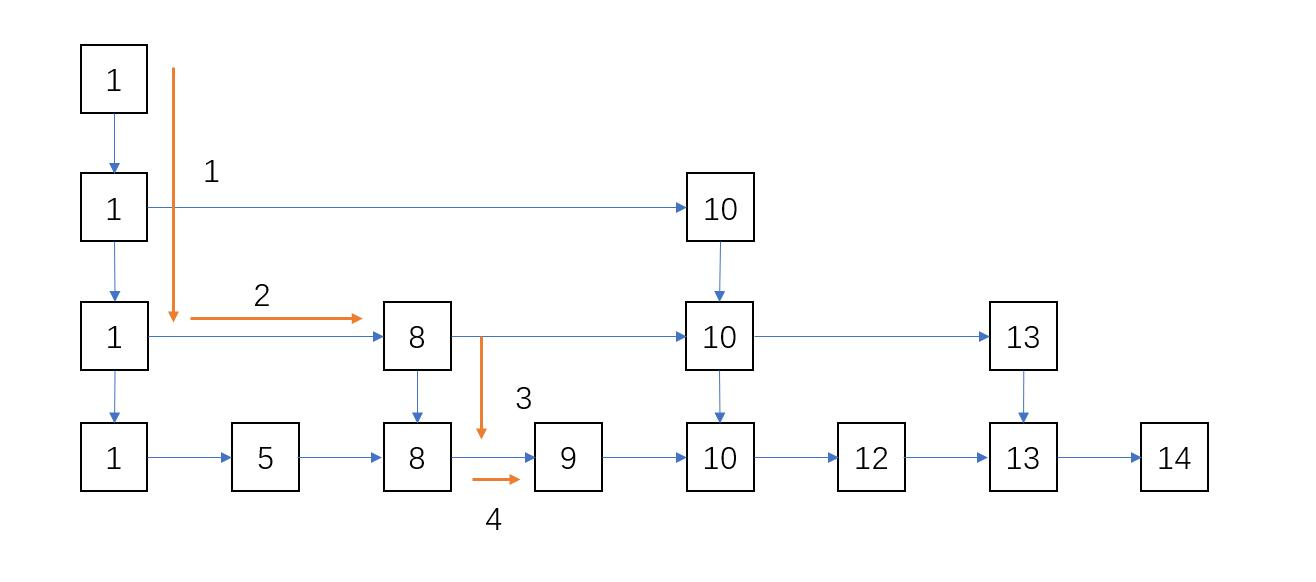
\includegraphics[scale=0.25]{./img/fasterter.jpg}
		\end{figure}
		\begin{enumerate}
			\item 查询是$O(\log n)$了! \quad \pause 可以证明每层横着走最多一次
			\pause
			\item 删除和加入都很困难
		\end{enumerate}
	\end{frame}
	\subsection{Skip List是怎么分块的}
	\begin{frame}
		\frametitle{Skip List是怎么分块的}
		\begin{figure}[H]
			\centering
			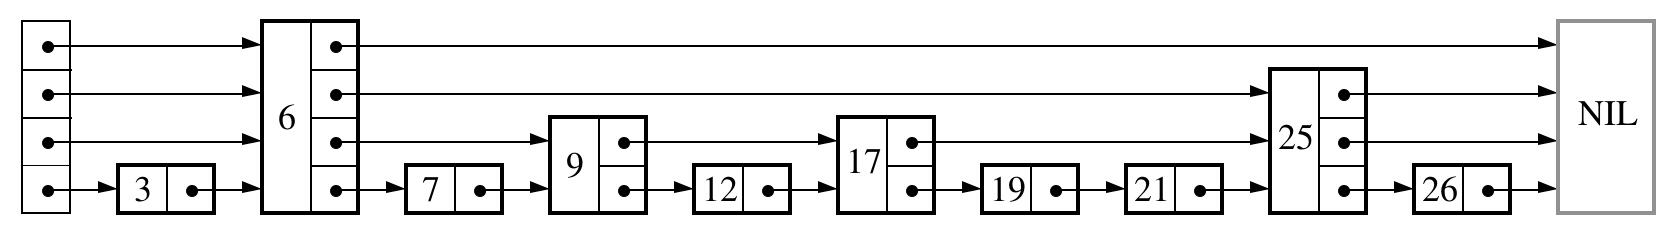
\includegraphics[scale=0.25]{./img/what_skip_list_is.jpg}
		\end{figure}
		通过高度来区分不同的块
	\end{frame}


	\begin{frame}
		\frametitle{Skip List是怎么分块的}
		\begin{algorithm}[H]
			\caption{getHeight}
			initialHeight $\leftarrow$ 0\;
			\While{initialHeight $<$ MAXVALUE and rand() $<$ p}{
				initialHeight $\leftarrow$ initialHeight + 1\;
			}
		\end{algorithm}
		一般将$MAXVALUE$设为$[\log{n}]$,将$p$设为0.5。
	\end{frame}

	\section{操作}
	\subsection{查找}
	\begin{frame}
		\frametitle{查找}
		\begin{figure}[H]
			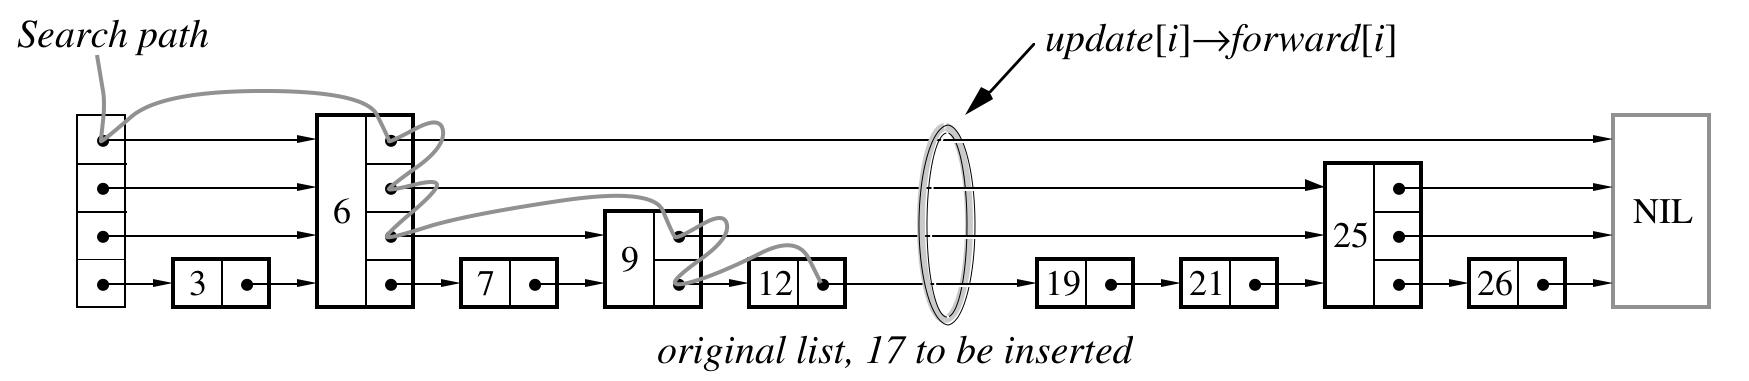
\includegraphics[scale=0.25]{./img/insert.jpg}
		\end{figure}
	\end{frame}

	\subsection{插入}
	\begin{frame}
		\frametitle{插入}
		\begin{figure}[H]
			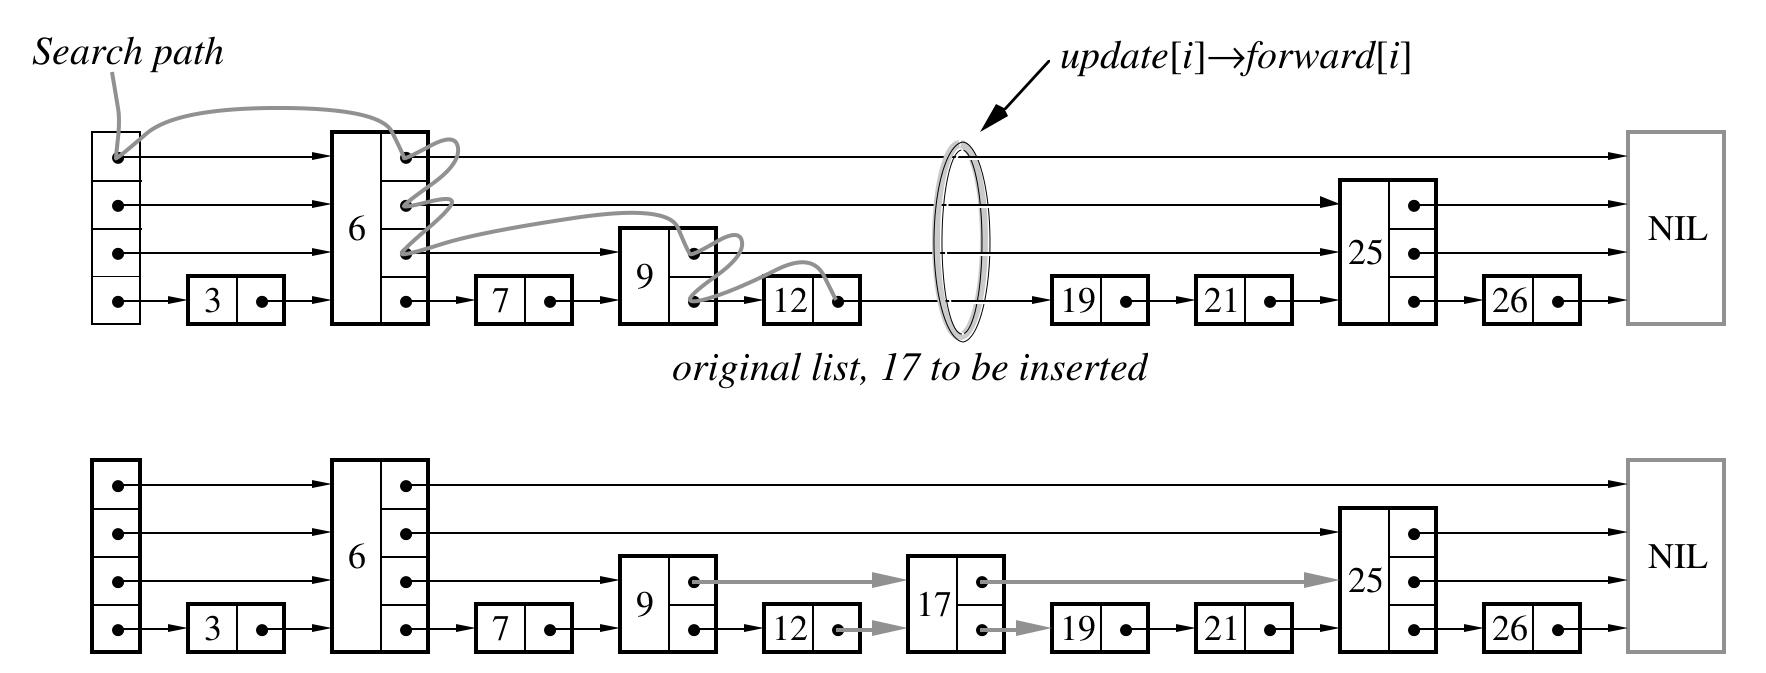
\includegraphics[scale=0.2]{./img/find.jpg}
		\end{figure}
	\end{frame}
	\subsection{删除}
	\begin{frame}
		\frametitle{删除}
		\begin{figure}[H]
			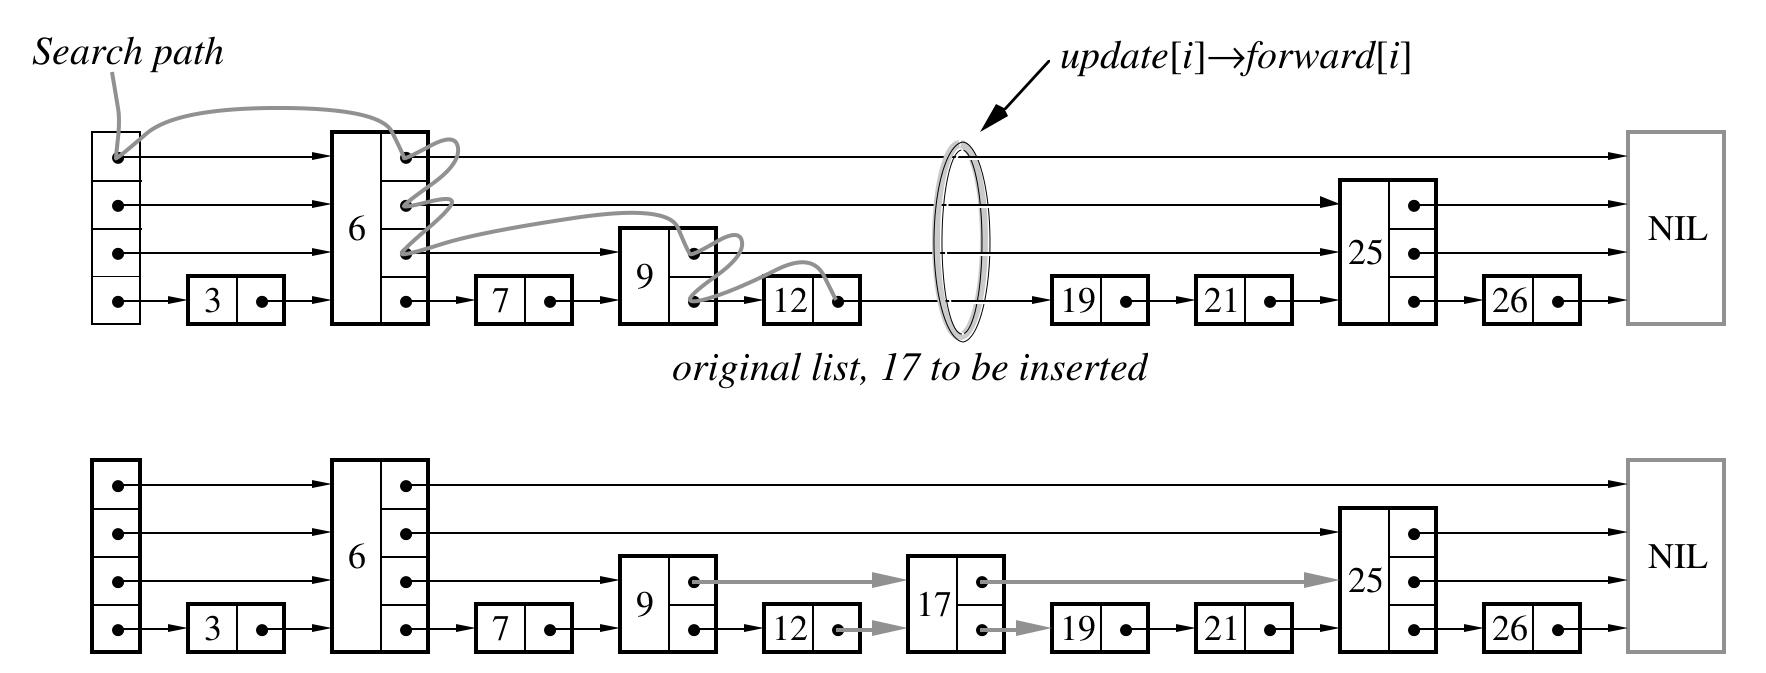
\includegraphics[scale=0.2]{./img/find.jpg}
		\end{figure}
	\end{frame}

	\subsection{rank}

	\begin{frame}
		\frametitle{求第$k$大}
		给每条边加权
		\begin{figure}[H]
			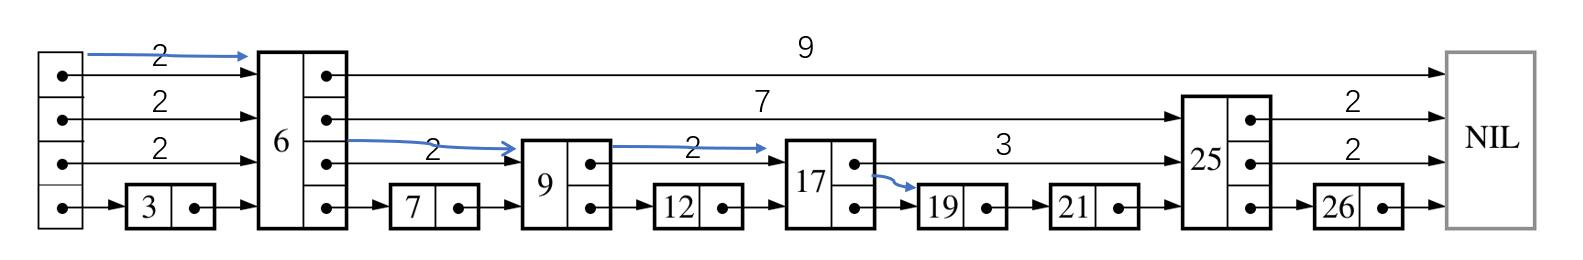
\includegraphics[scale=0.2]{./img/rank.jpg}
		\end{figure}
	\end{frame}

	\begin{frame}
		\frametitle{求第$k$大}
		此处应有一张rank tree的图。
	\end{frame}

	\begin{frame}
		\frametitle{求rank}
		我可以二分呀(X)
	\end{frame}

	\begin{frame}
		\frametitle{求rank}
		此处又应有一张rank tree的图。
	\end{frame}


	\begin{frame}
		\frametitle{求rank}
		累加每条边的长度
		\begin{figure}[H]
			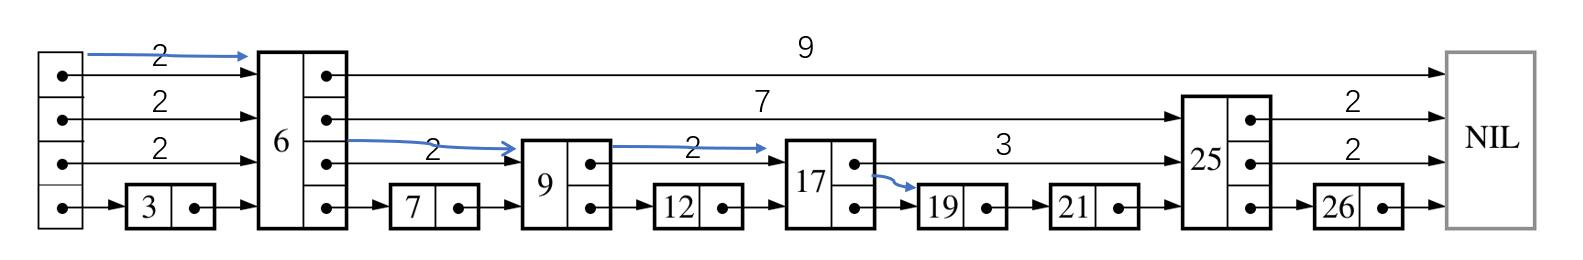
\includegraphics[scale=0.2]{./img/rank.jpg}
		\end{figure}
	\end{frame}


	


	\section{空间复杂度}
	\begin{frame}
		\frametitle{空间复杂度}
		$$E[X] = \sum_{i=1}^{n}E[X_{i}] = \sum_{i=1}^{n}\sum_{j=1}^{\infty}jp^{j} = \sum_{i=1}^{n}\frac{p}{(p-1)^2} = \frac{np}{(p-1)^2}$$
		取$p=\frac{1}{2}$,$E[X] = 2n$,期望空间复杂度$O(n)$ \\
		显然最坏情况下空间复杂度为$O(n\log n)$
	\end{frame}
	\section{时间复杂度}
	\begin{frame}
		\frametitle{先感性理解一下}
		\begin{figure}[H]
			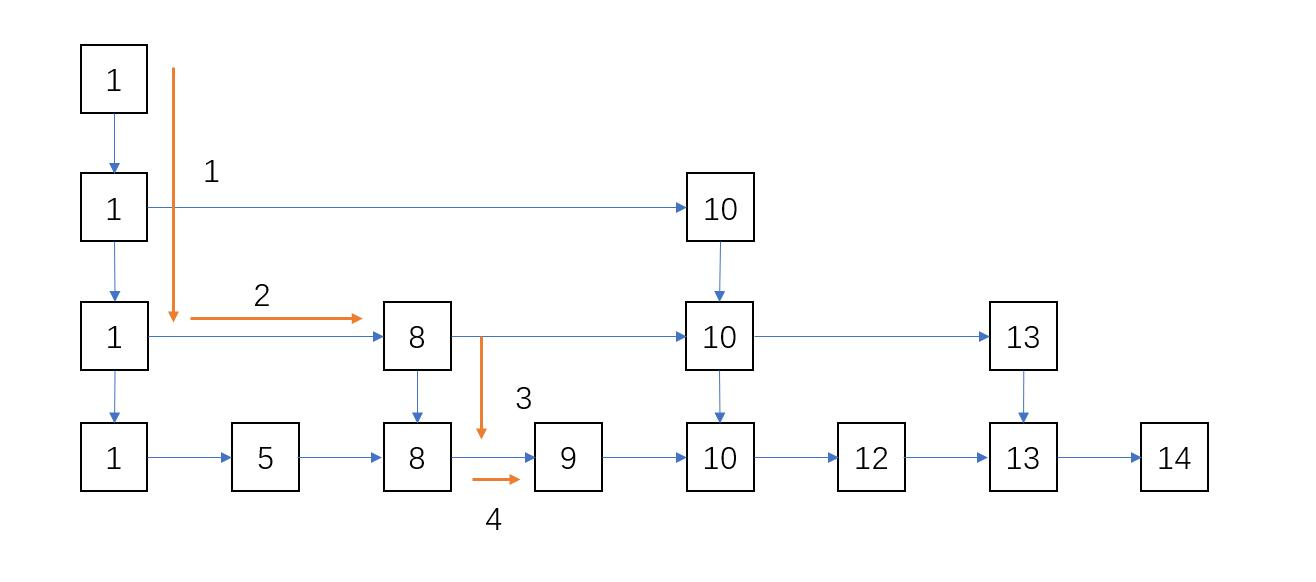
\includegraphics[scale=0.25]{./img/fasterter.jpg}
		\end{figure}
	\end{frame}
	\begin{frame}
		\frametitle{查找的复杂度}
		考虑反着思考复杂度
		\begin{enumerate}
			\item 跳到最高处的步数
			\item 跳到起点的步数
		\end{enumerate}
	\end{frame}
	\begin{frame}
		\frametitle{跳到最高处的步数}
		考虑一个无限长的Skip List
		\begin{figure}[H]
			\centering
			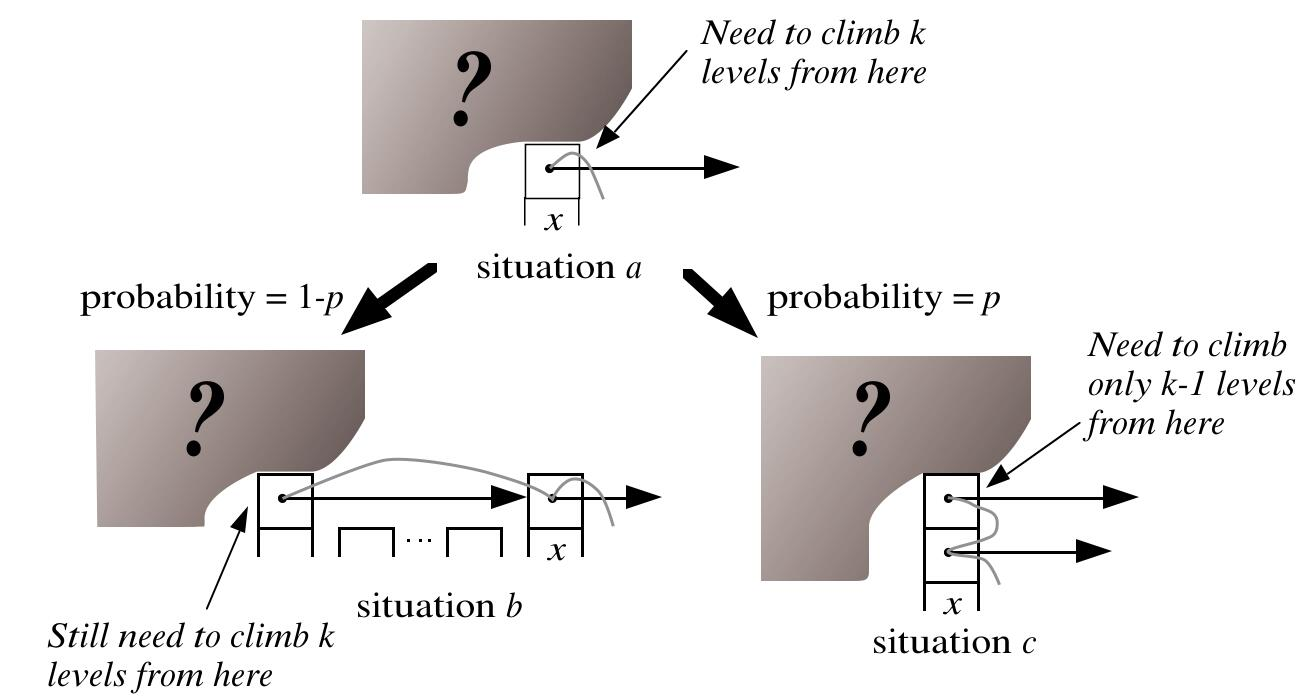
\includegraphics[scale=0.2]{img/complexity.jpg}
		\end{figure}
		\pause
		$$E[Y] = pE[Y]+(1-p)E[Y-1]+1$$
	\end{frame}
	\begin{frame}
		\frametitle{跳到最高处的步数}
		$$E[Y] = (1-p)E[Y]+pE[Y-1]+1$$
		\pause
		\\化简得\\
		$$E[Y] - E[Y-1] = \frac{1}{p}$$\\
		\pause
		$$E[0] = 0$$
		\pause
		于是$E[Y] = \frac{Y}{p}$
		\pause
		当$Y = [\log{n}]-1, p=\frac{1}{2}$,有$E[Y] = 2[\log{n}]-2$
	\end{frame}
	\begin{frame}
		\frametitle{跳到起点的步数}
		分析最高层有多少个数。
		$$E[Z] = \sum_{i=1}^{n}\sum_{j=[\log n]}^{\infty}jp^{j} 
		= \frac{np^{[\log{n}]} (p+[\log{n}]-p[\log{n}])}{(p-1)^2} $$
		\pause
		取$p=\frac{1}{2}$\\
		$$E[Z] \leq 2[\log{n}]+2$$
	\end{frame}
	\begin{frame}
		\frametitle{时间复杂度}
		\begin{enumerate}
			\item 跳到最高处的步数 \quad $E[Y] = 2[\log{n}]-2$
			\item 跳到起点的步数 \quad $E[Z] \leq 2[\log{n}]+2$
		\end{enumerate}
		期望复杂度为$O(\log{n})$ \\
	\end{frame}
	\begin{frame}
		\frametitle{$\Omega$ O $\Theta$的区别...}
		\begin{figure}[H]
			\centering
			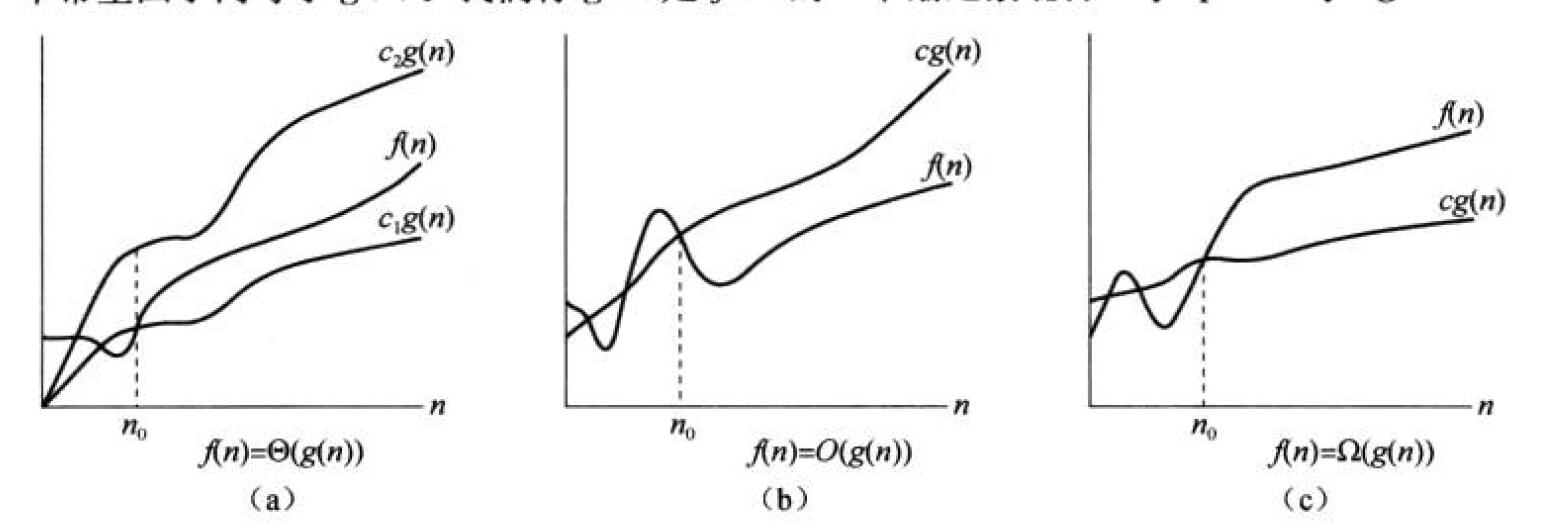
\includegraphics[scale=0.2]{./img/Ocomplexity.jpg}
		\end{figure}
		\pause
		其实这个跟最好最坏情况没什么关系...
	\end{frame}

	\begin{frame}
		\frametitle{时间复杂度}
		可以证明查找的复杂度在期望情况下是$\Theta(\log{n})$ \\
		但这并没有什么卵用,大家其实并不在乎$\Theta$和O
	\end{frame}
	\begin{frame}
		\frametitle{时间复杂度}
		\begin{enumerate}
			\item 查找 \quad 期望$O(\log n)$,最坏$O(n)$
			\item 插入 \quad 期望$O(\log n)$,最坏$O(n)$
			\item 删除 \quad 期望$O(\log n)$,最坏$O(n)$
			\item 前驱 \quad 期望$O(\log n)$,最坏$O(n)$
			\item 后继 \quad 期望$O(\log n)$,最坏$O(n)$
			\item 第$k$大 \quad 期望$O(\log n)$,最坏$O(n)$
			\item $rank$ \quad 期望$O(\log n)$,最坏$O(n)$
		\end{enumerate}
	\end{frame}
	\subsection{其他操作的复杂度}
	\begin{frame}
		\begin{enumerate}
			\item 插入 \quad 查找时维护每个高度最后的一个结点
			\item 删除 \quad 查找时维护每个高度最后的一个结点
			\item 前驱 \quad 本质就是查找
			\item 后继 \quad 查找之后跳到最底层再往前跳
			\item 第$k$大 \quad 本质就是搜索
			\item rank \quad 本质就是搜索
		\end{enumerate}
	\end{frame}

	\begin{frame}
		\frametitle{区间求和}
		\begin{figure}[H]
			\centering
			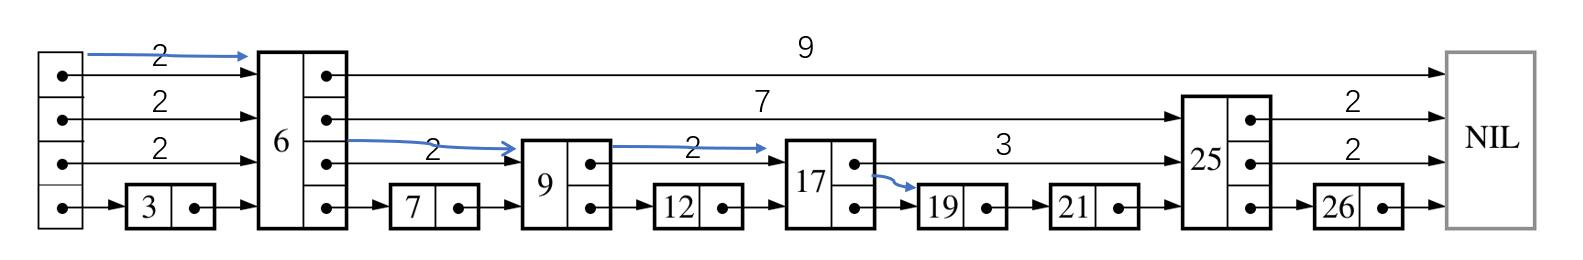
\includegraphics[scale=0.25]{./img/rank.jpg}
		\end{figure}
		求rank实际上就是一种弱的区间求和
	\end{frame}

	\begin{frame}
		\frametitle{并行}
		相比于普通平衡树,跳表每次要加锁的地方更少。
	\end{frame}

	\begin{frame}
		\frametitle{它是个链表}
		区间移动,文本编辑器。
	\end{frame}

	\begin{frame}
		\frametitle{可以用来实现ETT}
		\begin{enumerate}
			\item 欧拉序
			\item 动态树
			\item link-cut
			\item 维护子树信息
			\item 维护到根信息
		\end{enumerate}
	\end{frame}


	\section*{}
	\begin{frame}
		感谢倾听!
	\end{frame}
\end{document}